\begin{figure*}[p]
\centering
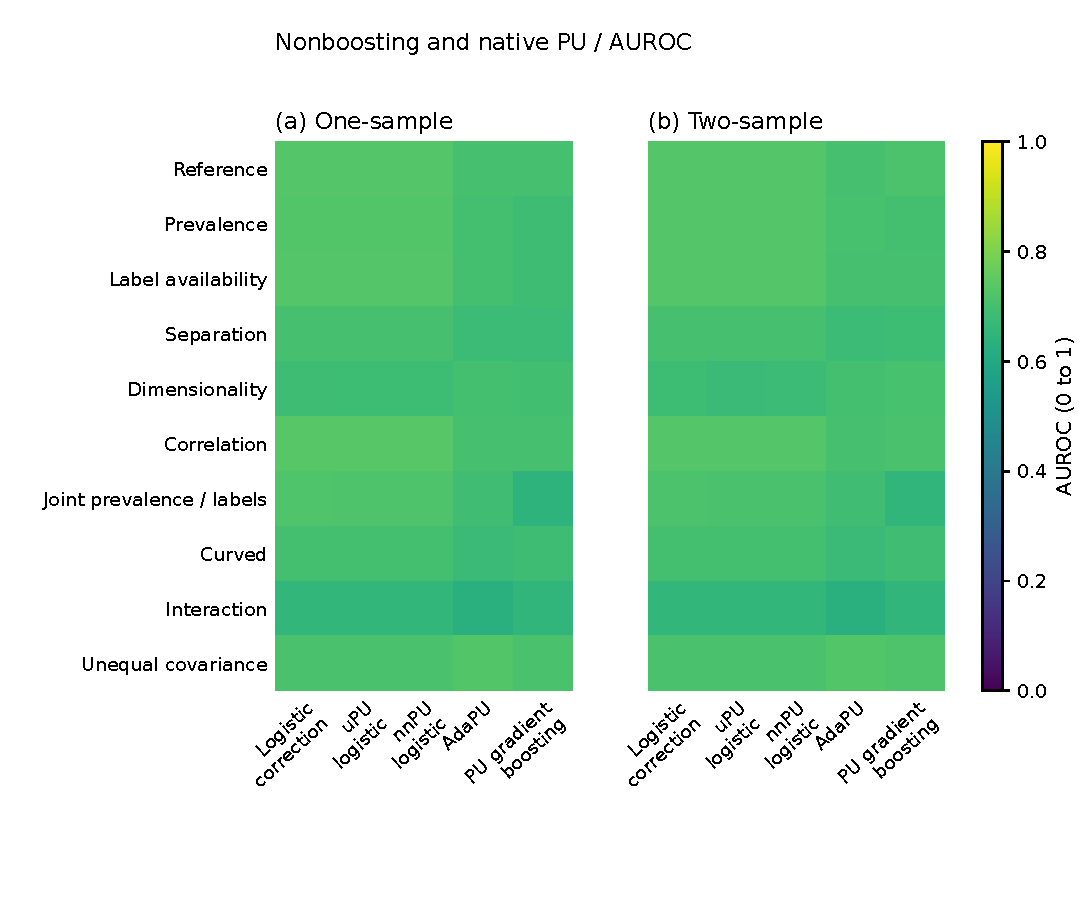
\includegraphics[page=1,width=\textwidth]{revised_figures/fig_s_core_full_fixed_methods.pdf}
\caption{Absolute AUROC and AP for all 25 PU configurations, split into prespecified method blocks. Values average settings within each of the ten families. Scales are identical (0 to 1) across designs and blocks; no group maximum is taken. Nonboosting and native PU / AUROC. Within-family means over settings; all 25 PU configurations retained across blocks.}
\label{fig:s-core-full-fixed-methods-1}
\end{figure*}
\begin{figure*}[p]
\centering
\includegraphics[page=2,width=\textwidth]{revised_figures/fig_s_core_full_fixed_methods.pdf}
\caption{Absolute AUROC and AP for all 25 PU configurations, split into prespecified method blocks. Values average settings within each of the ten families. Scales are identical (0 to 1) across designs and blocks; no group maximum is taken. Naive boosting / AUROC. Within-family means over settings; all 25 PU configurations retained across blocks.}
\label{fig:s-core-full-fixed-methods-2}
\end{figure*}
\begin{figure*}[p]
\centering
\includegraphics[page=3,width=\textwidth]{revised_figures/fig_s_core_full_fixed_methods.pdf}
\caption{Absolute AUROC and AP for all 25 PU configurations, split into prespecified method blocks. Values average settings within each of the ten families. Scales are identical (0 to 1) across designs and blocks; no group maximum is taken. Corrected boosting / AUROC. Within-family means over settings; all 25 PU configurations retained across blocks.}
\label{fig:s-core-full-fixed-methods-3}
\end{figure*}
\begin{figure*}[p]
\centering
\includegraphics[page=4,width=\textwidth]{revised_figures/fig_s_core_full_fixed_methods.pdf}
\caption{Absolute AUROC and AP for all 25 PU configurations, split into prespecified method blocks. Values average settings within each of the ten families. Scales are identical (0 to 1) across designs and blocks; no group maximum is taken. RN boosting / AUROC. Within-family means over settings; all 25 PU configurations retained across blocks.}
\label{fig:s-core-full-fixed-methods-4}
\end{figure*}
\begin{figure*}[p]
\centering
\includegraphics[page=5,width=\textwidth]{revised_figures/fig_s_core_full_fixed_methods.pdf}
\caption{Absolute AUROC and AP for all 25 PU configurations, split into prespecified method blocks. Values average settings within each of the ten families. Scales are identical (0 to 1) across designs and blocks; no group maximum is taken. CS boosting / AUROC. Within-family means over settings; all 25 PU configurations retained across blocks.}
\label{fig:s-core-full-fixed-methods-5}
\end{figure*}
\begin{figure*}[p]
\centering
\includegraphics[page=6,width=\textwidth]{revised_figures/fig_s_core_full_fixed_methods.pdf}
\caption{Absolute AUROC and AP for all 25 PU configurations, split into prespecified method blocks. Values average settings within each of the ten families. Scales are identical (0 to 1) across designs and blocks; no group maximum is taken. Nonboosting and native PU / AP. Within-family means over settings; all 25 PU configurations retained across blocks.}
\label{fig:s-core-full-fixed-methods-6}
\end{figure*}
\begin{figure*}[p]
\centering
\includegraphics[page=7,width=\textwidth]{revised_figures/fig_s_core_full_fixed_methods.pdf}
\caption{Absolute AUROC and AP for all 25 PU configurations, split into prespecified method blocks. Values average settings within each of the ten families. Scales are identical (0 to 1) across designs and blocks; no group maximum is taken. Naive boosting / AP. Within-family means over settings; all 25 PU configurations retained across blocks.}
\label{fig:s-core-full-fixed-methods-7}
\end{figure*}
\begin{figure*}[p]
\centering
\includegraphics[page=8,width=\textwidth]{revised_figures/fig_s_core_full_fixed_methods.pdf}
\caption{Absolute AUROC and AP for all 25 PU configurations, split into prespecified method blocks. Values average settings within each of the ten families. Scales are identical (0 to 1) across designs and blocks; no group maximum is taken. Corrected boosting / AP. Within-family means over settings; all 25 PU configurations retained across blocks.}
\label{fig:s-core-full-fixed-methods-8}
\end{figure*}
\begin{figure*}[p]
\centering
\includegraphics[page=9,width=\textwidth]{revised_figures/fig_s_core_full_fixed_methods.pdf}
\caption{Absolute AUROC and AP for all 25 PU configurations, split into prespecified method blocks. Values average settings within each of the ten families. Scales are identical (0 to 1) across designs and blocks; no group maximum is taken. RN boosting / AP. Within-family means over settings; all 25 PU configurations retained across blocks.}
\label{fig:s-core-full-fixed-methods-9}
\end{figure*}
\begin{figure*}[p]
\centering
\includegraphics[page=10,width=\textwidth]{revised_figures/fig_s_core_full_fixed_methods.pdf}
\caption{Absolute AUROC and AP for all 25 PU configurations, split into prespecified method blocks. Values average settings within each of the ten families. Scales are identical (0 to 1) across designs and blocks; no group maximum is taken. CS boosting / AP. Within-family means over settings; all 25 PU configurations retained across blocks.}
\label{fig:s-core-full-fixed-methods-10}
\end{figure*}
